\section{Function Follows Form Follows Function Follows Energy: Iron to Silicon, Steam to Cyber}

\underline{Observation}: Metamorphing boundaries between `engineering' and `designing' forms (as verbs) with regard to `scientific' and `artistic' reasoning (as adverbs)---philosophical, historical, practical, semantic, and neurological boundaries probably reckoned by the human capacitity to reason in both domains---puts potential designers in a steep quandary. On one hand, applying mathematics, physics, and logic to model particular systems enables forms and formalities capable of achieving end-states with relatively high fidelity and invariance. On the other hand, the capacity to reason about particular systems in all their chance, variability, and quality also permits an ability to bring about form, further appealing to the virtually ineffable design factors such as the historical, visual, spatial, or somatosensory.

Three historical lenses: structural art of the modern industrial revolutions, twentieth century modernism, and Eli Attia's modern framework of \textit{Engineered Architecture} envision epistemological and technical evolutions reflected on the interplay between `engineered' and `architectural' design forms, computation and intuition, artificial and natural, and technology and society. Considering a rough trajectory of design and designed forms across these worlds is to presuppose some historical grounds for the present potential to build one way or another.

\begin{flushright}
  \small{
  \textit{``In his 1957 book \textrm{The Reason of Structural Types}, Torroja wrote that ``Vain would be the enterprise of somebody who would propose himself to design a structure without having understood to the backbone the mechanical principles of inner equilibrium." Being an engineer, he saw those principles and their interiorization as something that was independent from history. I would like to challenge that position. For in the understanding of the backbone of the mechanical principles of inner equilibrium we are necessarily indebted to the way we perceive our body and its movements. In the past decades, cultural historians have multiplied sudies showing that this perception is to a certain extent a social construct. Gravity, just like a certain number of fundamental natural constraints, is always perceived through the prism of our body, a historically determined body."}} \\ --- Antoine Picon, Construction History: Between technological and cultural history
\end{flushright}

\clearpage

Before looking back, it is important to note that the lines of construction history also extend to a number of other theoretical histories and to an infinitude of real histories. Theorizing about history is only tangentially relevant to contemporary technological design, and moreso but seemingly diminishingly so to contemporary architectural design. At an even higher level, authors of construction history are usually also engineers and architects, with doctrinal responsibilities to write about it one way or another. \cite[p14]{CONSHISTORY} Here, consulting history to presuppose a grounds for building rammed-earth systems is directed towards the flux of concepts and methodologies rather than stylistic or technical precedents.

Furthermore, setting one endpoint in the early twenty-first century and expecting some level of detail permits only a sliver of building history. Ancient building history, the most relevant to earthen architecture, is postponed to a later section. But a latent continuity may reside if the eras prior to the eighteenth century possess the truly polytechnic heritage Lewis Mumford claims:

\begin{quote}
\small{
``Because the era before the eighteenth century is mistakenly supposed to have been technically backward, one of its best characteristics has been overlooked: namely, that it was still a mixed technology, a veritable polytechnics, for the characteristic tools, machine-tools, machines, utensils, and utilities it used did not derive solely from its own period and culture, but had been accumulating in great variety for tens of thousands of years. . . The introduction of new inventions like the clock did not necessitate on principle the discarding of any of these older achievements."} \cite[p134]{MYTHMACHINE}
\end{quote}

\subsection{Function Follows Form}

Designer, engineer, historian of technology, and professor David Billington provides an account of ``structural art" in \textit{The Tower and the Bridge}. According to Billington, structural art is a form of building tall structures, bridges, towers, long-span roofs, and similar objects of this structural class; originating in eighteenth-century Britain. A first epoch of structral engineering began with the industrialization of iron and this phenomenon's reflexive imperative to build more robust infrastructure, and concluded with the construction of the iron Eiffel Tower as the production of steel and reinforced concrete overran the construction world. A second epoch of structural art began in the 1800s and concluded around the assassination of Franz Ferdinand, when war appeared on the horizon and building stalled. \cite[p7]{TOWERANDBRIDGE}

Billington write of a discernible order in engineering/technology : science, structural : architectural design, and structures : machines summarized in the following:

\begin{enumerate}
  \item [] \textbf{Engineering and Science:} ``There is a fundamental difference between science and technology. Engineering or technology is the making of things that did not previously exist, whereas science is the discovering of things that have long existed. Technological results are forms that exist only because people want to make them, whereas scientific results are fomulations of what exists independently of human intentions. Technology deals with the artificial, science with the natural."\cite[p9]{TOWERANDBRIDGE}

  \item [] \textbf{Structures and Architecture:} ``Structural designers give the form to objects that are of relatively large scale and of single use, and these designers see forms as the means of controlling the forces of nature to be resisted. Architectural designers, on the other hand, give form to objects that are of relatively small scale and of complex human use, and these designers see forms as the means of controlling the spaces to be used by people." \cite[14]{TOWERANDBRIDGE}

  \item[] \textbf{Structures and Machines:} ``As intimitely connected as they are, structures and machines must function differently, they come into being by different social means, and they symbolize two distinctly different types of designs. Structures must not move perceptibly, are custom-built for one specific locale, and are typically designed by one individual. Machines, on the other hand, only work when they move, are made to be used widely, and are in the late twentieth century typically designed by teams of engineers. General statements about technology are frequently meaningless unless this basic distinction is made."\cite[p13]{TOWERANDBRIDGE}


\end{enumerate}

It becomes clear that the distinction made for structural art imposes boundaries on subjects and objects alike. What comes to be defined as an art form, separate but parallel to other forms of engineering and architecture, derives itself from higher epistemological movement as well as intricate technical realisms tied to all kinds of histories. Succinctly, Billington proposes a familiar principle emerging at the kernel of structural art:

\begin{quote}
  ``The first principle of structural art is that {\large{\textbf{the form controls the forces.}}} In general terms, this means that {\large{\textbf{function follows form}}}" \cite[p87]{TOWERANDBRIDGE}
\end{quote}

\begin{figure}[h!]
  \centering
  \fbox{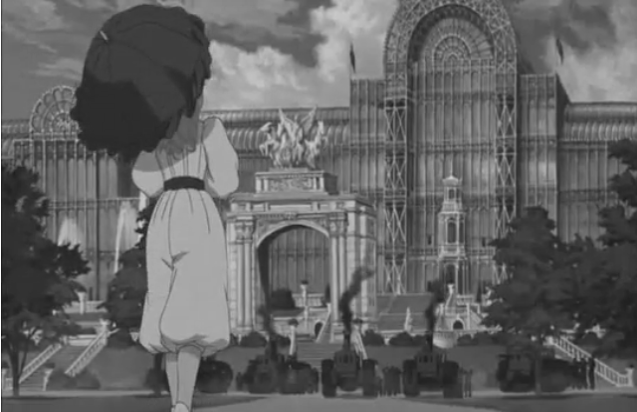
\includegraphics[scale=0.47]{crystalpalacebw.png}}
  \caption{Katsuhiro Otimoto and Sunrise's rendering of the Crystal Palace in the film \textit{Steamboy}, 2004. In quest of a revolutionary technology within, the British army destroys the palace. Similarly, in \textit{The Difference Engine}, a 1991 science-fiction novel by Gibson and Sterling, a Victorian-era warehouse is destroyed in quest of a set of computational punch-cards thought to predict gambling outcomes. Obviously, the potential for representing this world is artistically strong.}
\end{figure}

In order to rationalize these boundaries put forward by the lens of structural art, Tom F. Peters' \textit{``How the introduction of iron in construction changed and developed thought patterns in design"} is broadly referenced as a source for epistemological and technical patterns moving through this era. Three modes of thought: `overlay' thought \cite[36]{IRON} of pre-modern design, `model' thought \cite[37]{IRON} developing under the influence of the Enlightenment, and the `kit-of-parts' thought \cite[53]{IRON} leading into the twentieth century.

\textit{The overlay mode} of building appears between the ``veritable polytechnics" of pre-eighteenth century thought and the nucleation of a more structured, analytical form of polytechnics. It is a pre-theoretical idea, relying on a collective of experiential and experimental forms rather than analysis of structural behavior. `Overlay' implies the superposition of invented and analogous forms and methods directed towards the invention of progressively grander structures. The absence of analysis allows ``more flexible and redundant" structures, compared to calculated, deterministic paths. \cite[p36, 37]{IRON}





Iron was another of the ancient building materials acting at small scales as a mostly connective or tooling element. Industrialization cheapened the material while also ensuring its material consistency in mass production. \cite{IRON} From this alone, the subjects of structural art are solely concerned with the static object of structural design; belonging to a certain typological class, material, location, and scale.

A second epoch of structural art occurred in the 1880s with an explosion of steel and reinforced concrete. Exemplary of structural art built during this time was the Eiffel Tower. French artists reacted negatively to its construction, as it departed steeply from surrounding normal architecture and it was dark, dirty, and pompously gigantic. \cite{EIFFELTOWER} ``The works of structural art have sprung from the imagination of engineers who have, for the most part, come from a new type of school---the polytechnical school." \cite[p14]{TOWERANDBRIDGE} It is not far from here to recognize the pedagogical schism of architecture and technology embodied by separate French institutions: Ecole des Beaux-Arts and Ecole Polytechnique. \cite{SPACETIMEARCHITECTURE}

The technological innovations driving structural art followed from ``stretching" iron, steel, and concrete beyond successive limits, ``just as medieval designers had stretched stone into the skeletal Gothic cathedral." \cite[p5]{TOWERANDBRIDGE} Doing so enabled a rapid and reciprocating techno-social progress. However, this elasticism was not actually calculable until Claude-Louis Navier's theory of elasticity in the 1820's. \cite[p73]{RETROFITTINGMASONRY} Therefore, Billington claims that the engineering involved in structural art initially denied stress-related analyses for physical intuition and empiricism as its primary science. \cite[p43]{TOWERANDBRIDGE} In light of Mumford's conception of true polytechnics, the structural artists of the eighteenth century polytechnical school appear to be \textbf{the entrance for analytical rigor in building design.} THERMODYNAMICS ALSO on MECHANICAL SIDE


To handle the ethical pressures of government, shareholders, and industrialists idealizing the conservation of natural and public resources, in addition to the physical demands of building, three disciplines of structural art emerged to cover three dimensions of structure proposed by Billington. ``Efficiency, economy, and elegance" address the scientific dimension, the social dimension, and the symbolic dimension. \cite[p5,16,17]{TOWERANDBRIDGE}




It is conclusive from these propositions of the structural art that science and engineering are separate but parallel disciplines, similarly, structures and machines are separate but parallel objects, and structural design and architecture are separate but parallel disciplines as well. If the conversation between engineering and science is marked by conceptions of the artificial (variable) and conceptions of the natural (invariable), then a rift appears along the \textbf{system boundaries} of a model. System boundaries conceptually determine which quantities are of analytical concern and which are to be assumed external to the function of the system. If the conversation between structural design and architecture is marked by a physical object's magnitude and use, then a rift appears at \textbf{scaling}.

\begin{quote}
  ``The prototypical engineering form---the public bridge---requires no architect. The prototypical architectural form---the private house--- requires no engineer. We have seen that scientists and engineers develop their ideas in parallel and sometimes with much mutual discussion; and that engineers of structure must rely on engineers of machinery just to get their works built. Similarly, structural engineers and architects learn from each other and sometimes collaborate fruitfully, especially when, as with tall buildings, large scale goes together with complex use. But the two types of designers act predominantly in different spheres." \cite[p14]{TOWERANDBRIDGE}
\end{quote}






% \subsection{Knowledge}
% Begin etymologically with ``architecture": \textit{arkhi-} implying principal, chief, as in \textit{arche}trave, \textit{arche}gonium, \textit{Arch} Linux (a most skeletal Linux distribution); \textit{tekhne} implying art, craft, means, as in geo\textit{techn}ics, \textit{techn}ology, \textit{tec}tonics.
%
% Common to both mathematics and art is frequent appeal to the ancient West for insight, whether concerned with the roots of an Indo-European language, Euclid's axiomatic system, or Classical architectural orders. Classicism is productive in some cases, e.g. revisiting the Parallel Postulate, and hindering in others, e.g. the architectural debates on revivalism and ornamentation.
%
% reasoned about architecture as an art in the Nicomachean Ethics and wrote the following passage in the context of ``techne" as one of the chief intellectual virtues:
%
% \begin{quote}
% ``Now since architecture is an art and is essentially a reasoned state of capacity to make, and there is neither any art that is not such a state nor any such state that is not an art, \textit{art} is identical with a state of capacity to make, involving true reasoning. All art is concerned with coming into being i.e. with contriving and considering how something may come into being, i.e. with contriving and considering how something may come into being which is capable of either being or not being, and whose origin is in the maker and not in the thing made; for art is concerned neither with things that are, or come into being, by necessity, nor with things that do so in accordance with nature (since these have their origins in themselves). Making and acting are different, art must be a matter of making, not of acting. And in a sense chance and art are concerned with the same objects; as Agathon says, `Art loves chance and chance loves art'. Art then, as has been said, is a state concerned with making, involving true reasoning, and lack of art on the contrary is a state concerned with making, involving a false course of reasoning; both are concerned with the variable." \cite[p105]{NICOMACHEANETHICS}
% \end{quote}
%
% Mere observation of the etymological roots of ``architecture" shows that architecture, by definition, concerns a capacity to select (being and not being) and configure (consider and contrive) variables through true reasoning, but without explicity concerning scientific knowledge about these variables (not concerning nature or necessity) \textit{nor} empirical means of creation (making not acting). Scientific knowledge is reserved for the epistemic virtue of intellect, and practical means for the phronetic.
%
% \textit{Engineering}: from \textit{ingenium}, implying ability, cunning, inborn characteristics. Reliant on drawing from \textit{science}: from \textit{scire}, knowing, classifying, but as an intellectual virtue, without action.
%
% \begin{quote}
% ``Scientific knowledge is, then, a state of capacity to demonstrate, and has the other limiting characteristics which we specify in the Analytics, for it is when a man believes in a cetain way and the starting-points are known to him that he has scientific knowledge, since if they are not better known to him than the conclusion, he will have his knowledge only incidentally." \cite[p105]{NICOMACHEANETHICS}
% \end{quote}











% \subsection{Engineered Architecture}
% United States Patent Application US20090234696A1: ``Engineered Architecture" (EA); invented by Israeli-American architect/engineer Eli Attia and submitted in March of 2009. Per the Detailed Description of the Patent,
%
% \begin{quote}
%   ``A method [A system] of design, fabrication, and construction management, the method [system] comprising: receiving selections concerning a building shape and a building size; and executing instructions stored in memory of [a] computing device. . . determines that a plurality of design components are associated with the selected building shape and the selected building size, and generates a report concerning a building design comprising the determined plurality of design components." \cite{ATTIA2009EA}
% \end{quote}
%
% EA's method challenges the waste and inefficiency involved in the phasing of modern skyscrapers and other large buildings; coordination, communication, design, drawing, material provisioning, staffing, management, et cetera \cite{ATTIA2009EA}. By conceiving a library of structural components capable of composing structures determined by arbitrary constraints, the energy typically spent
%
%
%
% EA was never implemented in its intended form. In 2010, Attia partenered with Google X to realize EA at Google-scale. At the outset, it was predicted that the program could halve costs of building a commercial structure, revolutionize the accelerating need for urban construction globally, and reap around one hundred-twenty billion dollars in revenue for Google annually \cite{GLOBESEA}. By 2011 the patented work was ripped from Attia entirely; development continued minus the heart and brain of EA. As of March 2018, the debased mutation of EA, Flux, has stalled indefinitely \cite{FUCKFLUX}.




% Compared to current practice, EA claims a 44\% reduction in elapsed time from start of design to completion of construction, 52\% reduction of tasked items and services, 80\% earlier procurement of long-lead items, and 30\% reduction in cost and labor of an typical 30,000$m^2$ building.

% Following an invitation to share the idea with Google executives in 2010, the EA project was adopted by X, a research and development subsidiary of Alphabet Inc..  By 2014, Google had shouldered Attia out of the project and continued development of the software as ``Flux" \cite{GLOBESEA}.
%
%
%
%
%
%
% Here the modern building methodology is not intractably complex, it is artificially complicated.
%
% Most modern buildings may be perceived as layered assemblages of industrial products and painstakingly standardized procedures contrived for the rather elementary ends of physiological protection and psychrometric stability \cite[p88]{MOECONVERGENCE}. Historian Thomas Hughes' term ``technological momentum" renders the complicated accumulation of these technological contraptions engineered to fit socially constructed needs and their future reciprocities \cite{TECHNOMOMENTUM}. On the managerial side, principles of Scientific Management--- rationalized administration--- from the early twentieth century, settled into the architectural ethos during fervent reconstructive mode post-World War I \cite{MCLEODTAYLORISM}. Technological momentum, rationalized administration, and bureaucratic, corporated architecture are nailed into place during the Modernist rush following World War II \cite{KUBOCORPORATION}.
%
% Positivisms behind Computer Aided Design (CAD) and Building Information Modeling (BIM) pose  solutions for the design and construction industries through extradimensional modeling: real-time collaborative design in three dimensions, temporal sequencing along the fourth dimension, cost analysis as the fifth dimension, and lifecycle analysis as a sixth dimension \footnote{Richard McPartland, \textit{BIM dimensions - 3D, 4D, 5D, 6D BIM explained.} NBS. 10 July, 2017. \url{https://www.thenbs.com/knowledge/bim-dimensions-3d-4d-5d-6d-bim-explained}}.Ironically, CAD and BIM, deprived of
%
% \begin{quote}
%   ``An architectural agenda for energy ultimately requires a more fluxable program for buildings. By becoming more programmaticly inexact but in exacting ways, buildings characterized by precisely vague typologies and anticipitory functions can best trigger the emergent properties of actual complexity and the creative evolution of duration." \cite[p245]{MOECONVERGENCE}
% \end{quote}
%
%
% \begin{quote}
%   ``. . . analysis that identifies all involved material and energy flows from the formation of raw materials to end of life of the building." \cite[p. 70]{MOEHEA}
% \end{quote}
